\documentclass{article}
% \documentclass[10pt,a4paper]{elsarticle} % maye use this instead of the other
% one above

% package used :
\usepackage[utf8]{inputenc}
\usepackage[T1]{fontenc}
\usepackage{xspace}
\usepackage{graphicx}
\usepackage{svg}


\usepackage{todonotes}
\usepackage{paralist}
\usepackage{booktabs}
\usepackage{subfig}
\usepackage{comment}
\usepackage{algorithm}
\usepackage{algpseudocode}
\usepackage{multirow}
\usepackage{url}
\usepackage{amsmath,amsfonts,amsthm,paralist}
\usepackage{pstricks}
\usepackage[stable]{footmisc}
\usepackage{setspace,lipsum}
\usepackage{xcolor}
\usepackage{tabto}
\usepackage{ragged2e}
\usepackage{fullpage}

\usepackage[french]{babel}

% some command for custom font/style I guess
\newcommand{\ema}[1]{\ensuremath{#1}}
% \newcommand{\text}[1]{\textrm{#1}}

% "latin" abreviations
\newcommand{\ie}{\emph{i.e.,} }
\newcommand{\eg}{\emph{e.g.,} }
\newcommand{\cf}{\emph{\text{cf }}\xspace}
\newcommand{\etc}{\emph{etc}}

% Jargon informatique ici :
\newcommand{\cloud}{Cloud\xspace}
\newcommand{\clouds}{Clouds\xspace}
\newcommand{\api}{API\xspace}

% Initiales&Anagramme des entités
\newcommand{\CNRS}{CNRS\xspace}
\newcommand{\UCBL}{Université Claude Bernard Lyon 1\xspace}
\newcommand{\ENS}{École Normale Supérieure\xspace}
\newcommand{\LIP}{Laboratoire de l'Informatique du Parallélisme\xspace}
\newcommand{\INRIA}{\textsc{Inria}\xspace}
\newcommand{\MILYON}{MILYON\xspace}
\newcommand{\avalon}{AVALON\xspace}
\newcommand{\stack}{STACK\xspace}

% Programmes, Langages and such
\newcommand{\diet}{\textsc{Diet}\xspace} % recuperer les bonnes macros
\newcommand{\ns}{Naming Service\xspace}
\newcommand{\ma}{Master Agent\xspace}
\newcommand{\mas}{Master Agents\xspace}
\newcommand{\la}{Local Agent\xspace}
\newcommand{\las}{Local Agents\xspace}
\newcommand{\sed}{Server Daemon\xspace}

\newcommand{\concerto}{Concerto\xspace}

\newcommand{\gfivek}{Grid'5000\xspace}

\newcommand{\symphonyind}{Symphony in \diet} % xspace already here with \diet
\newcommand{\orchestrapi}{OrchestrAPI\xspace}

% beginning of the document
\begin{document}

\begin{titlepage}
	\begin{center}
		{\LARGE Université Claude Bernard Lyon 1}\\[2.5cm]
		\linespread{1.2}
		\huge {\bfseries Rapport de stage}\\
		{\large \emph{effectué au \LIP}}\\[1.5cm]
		\linespread{1}
		{\Large\bf Sylvère KANAPA}\\[1cm]
		{\large \emph{Tuteurs de stage:} Christian PÉREZ et Yves CANIOU}\\
		{\Large Étude du redéploiement du logiciel distribué \diet via
		l’environnement \concerto.}\\[0.5cm]
		{\Large Du 17/05/2021 au 23/07/2021}\\[1cm]
		\vspace{\fill}
		\today
	\end{center}

\end{titlepage}


\newpage
\section*{Remerciements}
À \textbf{Christian PÉREZ} et \textbf{Yves CANIOU}, mes maîtres de stage, pour
leurs conseils et leur patience au cours du stage.

% À \UCBL et \textbf{Mathieu MOY}, ma faculté et mon responsable de formation, de
% m'avoir donné l'oportunité de faire ce stage.

À \textbf{Binjamyn MAIRESSE}, un ami et collègue de stage pour les remarques et
discussions à propos du stage.

À \textbf{Clara PROTHET}, une amie qui a su me conseiller pendant mon stage et
mes études.

À mes amis, pour m'avoir encouragé et soutenu au cours de mes études et de ce
stage.


\newpage

\doublespacing
\tableofcontents

\newpage
\singlespacing
\section{Introduction}
%\subsection{Attentes du Stage :}
% introduire les systèmes distribués (DIET)

% introduire équipe stack
Avec le Fog/Edge computing\footnote{Paradigme informatique où les serveurs de
calculs et de stockage de données sont proches des sources qui les générent.},
le déploiement et la reconfiguration d’applications
distribuées\footnote{Logiciels et applications qui sont exécutés sur un système
distribué.} sur des systèmes distribués\footnote{Systèmes informatiques où les
différents éléments sont situés sur différentes machines reliées entre elles par
un réseau.} (tel que \diet\footnote{Logiciel distribué décrit dans la section
\ref{diet_section}.}) on connu une phase de complexification. Les équipes
projets \INRIA , \avalon et \stack, situées respectivement à Lyon et à Rennes, conduisent des
travaux afin de réaliser de telles opérations de manière sûre et très efficace.
Ces travaux ont amené à la réalisation de la preuve de concept
\concerto\footnote{Un logiciel permettant de l'orchestration automatique,
description dans la section \ref{concerto_section}}.
\diet est un système distribué qui permet distribuer des calculs sur des
ressources géographiquement distantes.
\concerto est un logiciel qui permet d'ordonnancer un logiciel ou un groupe de
logiciel en fonction de leurs étapes de fonctionnement.
Intégrer le logiciel distribué \diet dans l'environment \concerto permet de
simplifier son déploiement et sa reconfiguration dynamique.
La combinaison de ces deux logiciels a déjà été effectuée par le passé, mais ne
permettait pas de reconfigurations dynamiques de \diet.  C'est dans ce but que
notre travail nous a conduit à proposer une \api pour étendre les
fonctionnalités de \concerto, \orchestrapi, et à développer \symphonyind, une
intégration de \diet dans \concerto en utilisant \orchestrapi, qui permet la
reconfiguration dynamique.

% rajout d'information

\section{Présentation de l'entité d'accueil}

\subsection{\LIP}
Le \LIP réunit une centaine d'enseignants-chercheurs et doctorants en thèse
autour de différents sujets et problématiques de domaines divers de
l'informatique tels que le calcul arithmétique, les architectures logicielles,
les preuves de programmes.

Le \LIP est associé à diverses structures de recherche et d'enseignements. Ces
structures sont : le \CNRS, l'\ENS de Lyon, l'\INRIA et l'\UCBL. Le laboratoire
fait partie du \MILYON, un groupement de laboratoires situés à Lyon et
Saint-Étienne, composé de 350 chercheurs en informatique et mathématiques et
permettant de développer la recherche interdisciplinaire.

Le but du \LIP est d'étudier les fondements de l'informatique actuels puis
d'inventer de nouveaux concepts dans les domaines ciblés et d'en  mesurer les
répercussions dans les autres branches scientifiques.
Le laboratoire est dirigé par Nicolas Trotignon et subdivisé en 3 entités :
\begin{itemize}
	\item L'équipe administrative
	\item Les équipes de recherches
	\item Les moyens informatiques
\end{itemize}

Les équipes de recherche sont au nombre de 7 et chacune réalise des études dans
un ou plusieurs domaines informatiques. Celles-ci s'articulent généralement
autour de leurs spécificités :
\begin{itemize}
	\item  AriC : \emph{Calcul arithmétique}
	\item  \avalon : \emph{Algorithmes et architectures logicielles pour
	les plateformes distribuées et HPC}
	\item  CASH : \emph{Compilation et analyse, logiciel et matériel}
	\item  DANTE : \emph{Approche de capture temporelle et structurelle}
	\item  MC2 : \emph{Modèles de calcul, complexité, combinatoire}
	\item  PLUME : \emph{Programmes et Preuves}
	\item  ROMA : \emph{Optimisation de ressources}
\end{itemize}

\subsection{L'équipe de recherche \avalon}\label{equipe_avalon}

Au cours de ce stage, j'ai intégré l'équipe \avalon dirigée par Christian Pérez.
Les recherches d'\avalon s'orientent autour de 3 axes majeurs.

Premièrement, l'efficacité énergétique et la réduction de la consommation
d'énergie sont devenues  des enjeux importants dans divers secteurs industriels
et économiques et les systèmes informatiques  n'y échappent pas. Le but est de
développer des mécanismes et d'améliorer les analyses pour développer des
plateformes à grande échelle plus éco-responsables.

Deuxièmement, la compléxité des machines et applications tend à augmenter et
rend leurs éxécutions plus difficiles à gérer. Le but est de développer des
modèles qui permettent de décrire les structures de ces applications permettant
des éxécutions plus efficaces.

Troisièmement, l'équipe effectue des recherches autour de l'ordonnancement et la
mise en correspondance de processus avec les machines à disposition dans le
\cloud à grande échelle et de la recherche sur le traitement de flux données, la
gestion autonome de ressources dans des \clouds multiples, \dots

L'équipe est composée d'une dizaine d'enseignants-chercheurs et de 4 membres du
personnel parmis lesquels des assistants adminitratifs et des chercheurs. À cela
se joint une dizaine d'étudiants effectuant leur thèse au sein de l'équipe.

\section{Présentation du stage}
\subsection{Objectif du stage}

L’objectif du stage est de réaliser une étude de cas sur la pertinence du
logiciel \concerto\footnote{
\url{https://gitlab.inria.fr/VeRDi-project/concerto}} ainsi que d’implémenter
des fonctionnalités manquantes éventuelles.
Ainsi, nous utiliserons le déploiement et la reconfiguration dynamique de
\diet\footnote{\url{https://graal.ens-lyon.fr/DIET}} comme étude de cas.

%\diet, une implémentaion de GridRPC, sera utilisée comme étude de cas à déployer
%et à reconfigurer.

Le stage s'est déroulé en plusieurs sous-objectifs :
\begin{itemize}
	\item La prise en main de \diet – compilation et lancement à la main d’un
	exemple démo (fourni par \diet)

	\item La mise en \oe uvre d’un déploiement de \diet via un script dédié

	\item La définition et la mise en \oe uvre de scénario de reconfiguration de
	\diet

	\item La prise en main des concepts liés au déploiement et à la
	reconfiguration, et en particulier de l'environnement \concerto

	\item L’implémentation de fonctionnalités manquantes éventuelles à \concerto

	\item Le déploiement sur des conteneurs Docker
	% pas tout à fait, mais j'ai un dockerfile spécial pour diet!

	\item La réalisation d’expériences sur \gfivek\footnote{
	\url{https://www.grid5000.fr}}

\end{itemize}


\subsection{Cadre du travail}

% rajout d'un petit texte d'introduction pour dire que le stage était en
% télétravail (utilisation d'outils colaboratif) ?

\subsubsection{\gfivek}
\gfivek est un parc de serveurs dédié à la recherche scientifique dans
l'informatique. Voici une citation provenant de la page de présentation du
projet qui résume comment \gfivek est utilisé :
\begin{quotation}
	\og \gfivek est une plateforme d'essais à grande échelle orientée dans
	l'expérimentation scientifique dans tous les domaines de l'informatique, avec
	un focus sur les calculs parallèles et distribués incluant le \cloud
	(computing), HPC\footnote{High-Performance Computer}, Big-Data\footnote{\og
	Méga-Données \fg} et l'IA\footnote{Intelligence Artificielle}. \fg
\end{quotation}

\subsubsection{\diet}\label{diet_section}
\diet\cite{papier_diet} a été developpé par plusieurs membres de l'équipe
\avalon. Il permet de distribuer dynamiquement des problèmes sur des serveurs
capables de les résoudre.
% comme présenté dans la figure \ref{fig:diet_schema}.

\begin{figure}[h!]
\centering
	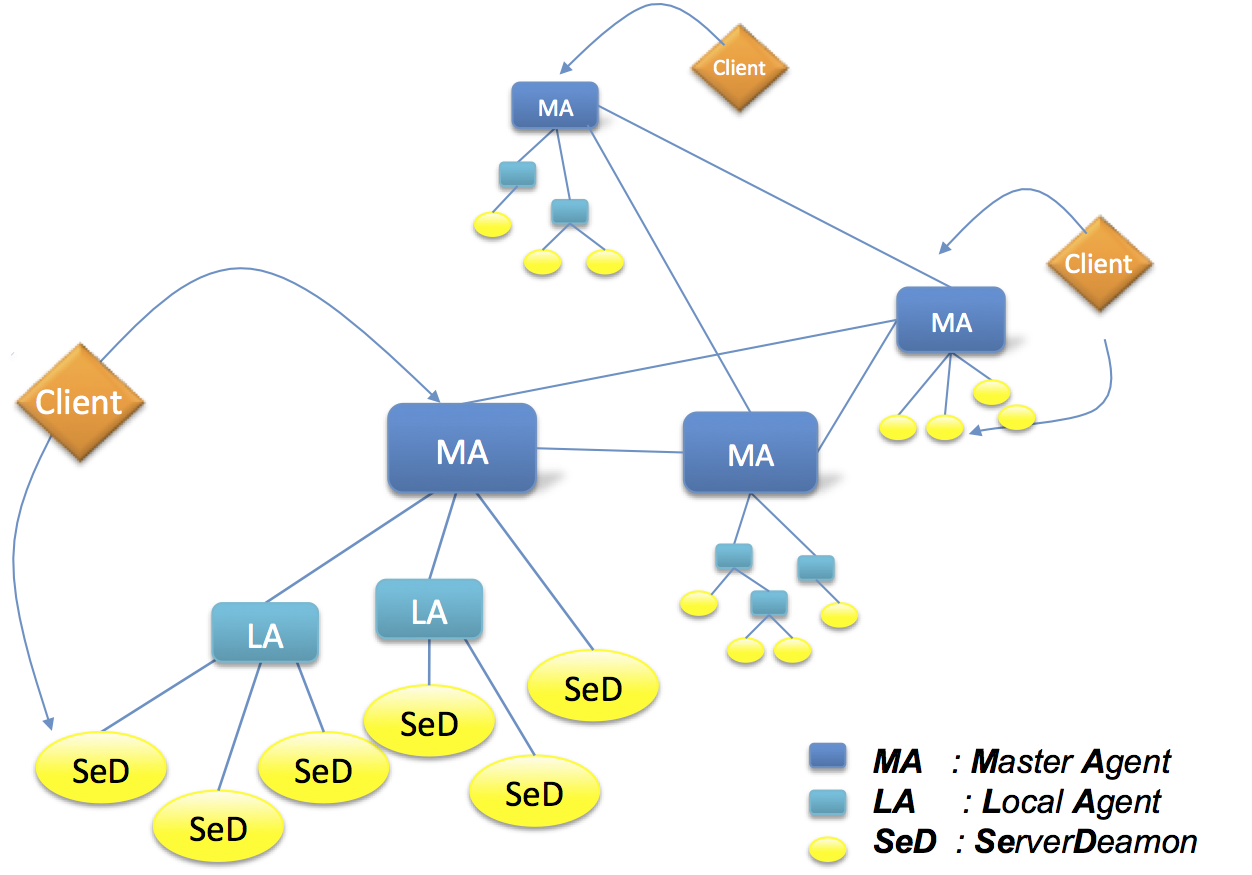
\includegraphics[scale=0.5]{../doc/diet_schema.png}
\caption{Une hierarchie d'Agents \diet}
\label{fig:diet_schema}
\end{figure}

% \diet utilise une architecture avec une hierarchie pour distribuer efficacement
% les problèmes:


Dans la figure \ref{fig:diet_schema}, on peut y voir une hierarchie \diet
déployée. Les différents éléments de cette hierarchie sont :
\begin{itemize}
	\item Client : Un client est une application \diet développée capable de
	résoudre des problèmes à distance. Une grande partie des différents types de
	clients sont capables de se connecter à un réseau \diet depuis une page web, un
	PSE\footnote{Power System Engineering} tel que Matlab\footnote{
	\url{https://www.mathworks.com/products/matlab.html}} ou Scilab\footnote{
	\url{https://www.scilab.org/}}, ou depuis un programme compilé.

	\item \sed : Un \sed encapsule un server de calculs. Par exemple il peut être
	situé au point d'entrée d'un ordinateur parallèle. Un \sed peut sauvegarder
	différentes informations, par exemple une liste de tous les problèmes qui
	peuvent être résolus dessus et/ou des informations en relation des
	performances telles que la quantité de mémoire disponible ou le nombre de
	ressources disponibles. Quand il s'enregistre, un \sed déclare les problèmes
	qu'il peut résoudre à son parent \la ou \ma.
	% Un \sed peut donner des informations à propos du matériel et des performances
	% en utilisant le module CoRI ou de la prédiction de performance pour certains
	% type de problèmes en utilisant le module CoRI.

	\item \la : Un \la transmet les requêtes au sein de l'arborescence/hierarchie
	\diet. Un \la sauvegarde la liste des services disponibles dans la
	sous-arborescence : pour chaque service, le \la sauvegarde/enregistre une
	liste de ses enfants (Agents et \sed) qui peuvent être contactés pour trouver
	le service. En fonction de la topologie du réseau sous-jacent, une hierarchie
	de \las peut être déployée entre le \ma et les \sed. La fonction d'un \la est
	aussi de faire de l'ordonnancement partiel sur sa sous-arborescence, ce qui
	reduit la quantité de travail pour le \ma.

	\item \ma : Un \ma est un \la particulier : celui-ci fait le lien entre la
	hierarchie \diet (particulièrement le \sed nécessaire) et le Client. La
	référence du \sed choisi est renvoyé au Client qui pourra se connecter
	directement au \sed. Un Client peut obtenir une référence au \ma par un nom
	de serveur spécifique ou une page web qui contient les différentes
	localisations des \mas.

\end{itemize}


De plus, pour interconnecter les Agents par un réseau, il faut gérer leurs noms. Pour
cela, nous utilisons un \og \ns \fg. Dans le cas de \diet,
CORBA\footnote{\url{https://corba.org/}} est utilisé.

% rajouter un schéma pour la s-s-section en dessous
\subsubsection{\concerto}\label{concerto_section}
\concerto a été developpé en Python par Maverick Chardet dans le cadre de sa
thèse~\cite{papier_concerto}, et est une extension du modèle de
Madeus~\cite{papier_madeus}. Il permet de coordonner un logiciel (ou un groupe de
logiciels) et de permettre l'automatisation de son lancement.

% définir un composant concerto

Un \og Composant \fg représente en général un module d'un logiciel distribué,
mais peut représenter n'importe quoi tant que son interface (les services et
données nécessaires à son fonctionnement et les services et données fournis)
peut être exprimée de manière explicite. Un Composant définit un cycle de vie
de la même manière qu'un automate\footnote{
\url{https://en.wikipedia.org/wiki/Transition_system}} (ou un réseau de
Petri\footnote{\url{https://en.wikipedia.org/wiki/Petri_net}}).

% Definition disponible dans la doc de concerto :

% Each component also defines a life-cycle represented as a state-machine
% (possibly presenting parallel transitions like Petri-nets). A place (a state of
% the state-machine) represents a milestone in the life-cycle of the component. A
% transition between two places allows a token (which marks a currently active
% place) to go from one place to another by executing an action tied to the
% transition. In this implementation, an action is a Python function. Transitions
% are labeled with a behavior. A transition can only be executed if it is labeled
% by the current active behavior of the component. The ports of a component are
% bound to places, transitions or groups of places to indicate that a service/data
% is used/provided when the corresponding place, transition or group is active. A
% group is active if there is at least one token in one of the places it contains
% or one of the transitions going from one place it contains to another place it
% also contains.

Ces Composants sont définis par différents éléments qui doivent être instanciés
par l'utilisateur de \concerto :
\begin{itemize}
	\item \texttt{places} : statut du logiciel, varie entre différentes étapes
	(exemple : \emph{Installé, Configuré, Éteint, Démarré})

	\item \texttt{groups} : l'union de plusieurs étapes (exemple : \emph{
	Démarrable : Configuré, Éteint})

	\item \texttt{transitions} : représentent les transitions entre les étapes
	(exemple : \emph{Installation, Configuration, Démarrage, Extinction})

	\item \texttt{dependencies} : représentent des \og ports \fg qui peuvent être
	connectés avec d'autres. Les \texttt{dependencies} bloquent l'exécution d'une
	transition tant que la dépendance n'est pas satisfaite (connectée, ou dans
	l'attente qu'une information soit transmise à travers ces ports)(exemple :
	\emph{Machine-Mère (Démarré : Est\_Démarrée), Machine-Fille (Démarrage :
	Machine\_Mère\_Démarrée)})

	\item \texttt{behaviors} : représentent une suite de transitions à effectuer
	les unes à la suite des autres (exemple : \emph{Déploiement : Installation,
	Configuration, Démarrage})

\end{itemize}

\emph{Pour un exemple d'un Composant instancié, voir les Figures
\ref{fig:naming_service} à \ref{fig:server_daemon}. Pour la légende, se réferrer
à la Figure \ref{fig:legende_schema}.}

Les dépendances peuvent être liées via l'\og Assemblage \fg avec d'autres
dépendances venant d'autres composants (il y a des dépendances
d'utilisation/d'usage et de provision, les premières doivent être connectées aux
secondes pour être satisfaites, les secondes ne sont pas obligatoirement
connectées pour être satisfaites). L'\og Assemblage \fg est la mise en relation
de différents Composants permettant un ordonnancement automatique des
transitions. Une fois assemblés et un \og Comportement \fg demandé, les
composants se lancent dès que possible en respectant les dépendances. Les
dépendances non satisfaites provoquent une attente passive\footnote{Une forme
d'attente où le Système d'Exploitation signale lorsque l'attente prend fin,
celle-ci ne prend pas de temps processeur.}.


\section{Une extension à l'\api de \concerto : \orchestrapi}\label{section:orchestrapi}
\subsection{Introduction} % une intro annonce une vue generale
\concerto est un outil qui permet de faire de l'orchestration, mais il ne
propose pas de solution pour déployer les fichiers nécessaires au fonctionnement
du (ou des) logiciel importé, ni pour permettre le déploiement à distance d'un
logiciel.

\orchestrapi\footnote{\url{https://gitlab.inria.fr/skanapa/orchestrapi}} permet
d'étendre les fonctionnalitées de \concerto, le tout en laissant une interface
plus simple à programmer et des interactions intégrées avec le système, notament
la gestion/déploiement de fichiers.
% être plus précis


\subsection{Description d'\orchestrapi}
Voici une liste des méthodes disponibles dans l'\api, celles-ci étendent les
fonctionnalités de l'\api de \concerto :
\begin{itemize}
	\item \texttt{get\_path()} : retourne le répertoire de travail de l'\api

	\item \texttt{get\_hostname()} : retourne le nom de l'hôte sur laquelle
	l'\api est appelée

	\item \texttt{write\_script(var\_export, cmdline, filename, gen\_pid\_file)}
	: permet d'écrire la commande passée en paramètre dans un script pour une
	exécution ultérieure

	\item \texttt{async\_files\_transfer(source, destination, rsync\_queue)} :
	permet d'ajouter la source et la destination (locale ou distante) d'un
	fichier à une queue

	\item \texttt{flush\_files\_transfer()} : permet de vider la queue en
	transférant tous les fichiers qu'elle contient

	\item \texttt{transfer\_files(source, destination)} : permet de transférer
	directement des fichiers

	\item \texttt{run\_cmd(cmdline)} : permet de lancer une simple commande en
	local ou sur une machine distante

	\item \texttt{kill\_scripted\_cmd(scriptname)} : est un \og wrapper \fg de la
	commande Unix \og kill\footnote{Commande qui permet d'envoyer un signal à un
	processus, notament pour l'arrêter.} \fg

\end{itemize}

En plus de ces méthodes, \orchestrapi étant une Classe, elle posséde des données
membres permettant d'articuler ses méthodes autour de l'usage voulu par
l'utilisateur. Des exemples sont fournis dans la section
\ref{apport_orchestrapi}.

% le paragraphe est moyen, à modifier


\section{\symphonyind : une intégration de \diet dans \concerto}\label{section:symphonyind}
\subsection{Introduction}
\symphonyind\footnote{
\url{https://gitlab.inria.fr/skanapa/symphony-in-diet}} est l'intégration de
\diet dans \concerto que j'ai développée en reprenant les travaux déjà effectués
avec \og Concerto-Diet \fg, \og Mad-Remote \fg et \og Mad-Diet \fg , qui sont
des anciennes intégrations de \diet dans \concerto ou une extension de l'\api de
\concerto. Ces projets datent de plusieurs années, et ne permettaient
respectivement pas de faire une reconfiguration dynamique de \diet, ni d'étendre
et de simplifier l'\api de \concerto. Ceux-ci ayant été développés en Python,
\symphonyind fut développé de même.


La première étape de conception a été de revoir les étapes et transitions des
composants de \diet de manière à prendre en compte une reconfiguration
dynamique, \ie modifier la configuration de l'arborescence de \diet sans avoir à
redémarrer toute une infrastructure \diet. Pour ce faire, chaque composant a eu
sa propre implémentation dans \symphonyind.

\symphonyind est une intégration des différents agents de \diet ainsi que d'un
\ns dans \concerto, il ne permet pas un assemblage automatique des composants.


% explication de comment on passe de diet à des composants de concerto par diet
\subsection{Description des composants}
Chaque Agent de \diet ainsi que le Naming Service a son composant dans
\symphonyind. Chaque composant différe  des autres car les Agents \diet n'ont
pas les mêmes étapes de fonctionnements, par exemple (\cf Figure
\ref{fig:naming_service} à Figure \ref{fig:server_daemon}): \newline\newline

\begin{minipage}{\textwidth}
	\centering
	\includesvg[scale=0.35]{../doc/template.svg}
	\captionof{figure}{Légende des schémas}
	\label{fig:legende_schema}
\end{minipage}\newline\newline


\hspace{0.05\textwidth}
\begin{minipage}{0.40\textwidth}
	\centering
	\includesvg[scale=0.35]{../doc/naming_service.svg}
	\captionof{figure}{Intégration du \ns en un composant \concerto}
	\label{fig:naming_service}
\end{minipage}
\hspace{0.05\textwidth}
\begin{minipage}{0.40\textwidth}
	\centering
	\includesvg[scale=0.35]{../doc/master_agent.svg}
	\captionof{figure}{Intégration du \ma en un composant \concerto}
	\label{fig:master_agent}
\end{minipage}\newline\newline

\hspace{0.05\textwidth}
\begin{minipage}{0.40\textwidth}
	\centering
	\includesvg[scale=0.35]{../doc/local_agent.svg}
	\captionof{figure}{Intégration du \la en un composant \concerto}
	\label{fig:local_agent}
\end{minipage}
\hspace{0.05\textwidth}
\begin{minipage}{0.40\textwidth}
	\centering
	\includesvg[scale=0.35]{../doc/server_daemon.svg}
	\captionof{figure}{Intégration du \sed en un composant \concerto}
	\label{fig:server_daemon}
\end{minipage}\newline\newline



% ANCIEN AFFICHAGE

% \begin{figure}[h!]
% 	\centering
% 		\includesvg[scale=0.4]{../doc/template.svg}
% \caption{Légende des schémas}
% \label{fig:legende_schema}
% \end{figure}
%
% \begin{figure}[h!]
% \centering
% 	\includesvg[scale=0.4]{../doc/naming_service.svg}
% \caption{Intégration du \ns en un composant \concerto}
% \label{fig:naming_service}
% \end{figure}
%
% \begin{figure}[h!]
% \centering
% 	\includesvg[scale=0.4]{../doc/master_agent.svg}
% \caption{Intégration du \ma en un composant \concerto}
% \label{fig:master_agent}
% \end{figure}
%
% \begin{figure}[h!]
% \centering
% 	\includesvg[scale=0.4]{../doc/local_agent.svg}
% \caption{Intégration du \la en un composant \concerto}
% \label{fig:local_agent}
% \end{figure}
%
% \begin{figure}[h!]
% \centering
% 	\includesvg[scale=0.4]{../doc/server_daemon.svg}
% \caption{Intégration du \sed en un composant \concerto}
% \label{fig:server_daemon}
% \end{figure}



\begin{itemize}
	\item Dans le schéma du composant \ns que l'on peut voir dans la Figure
	\ref{fig:naming_service}, figurent 3 \texttt{places}, 3 \texttt{transitions},
	2 \texttt{dependencies} de provisions, ainsi que l'union des \texttt{places}
	\og running \fg et \og configured \fg qui forment un \texttt{group}.\newline

	\item Le composant \ma, Figure \ref{fig:master_agent} est sensiblement le
	même que le composant \ns, les différences étant les binaires exécutés et 2
	\texttt{dependencies} d'usage supplémentaires pour le composant \ma.\newline

	\item Le composant \la, Figure \ref{fig:local_agent}, comporte 4
	\texttt{places}, 5 \texttt{transitions}, 6 \texttt{dependencies} dont 4
	d'usage et 2 de provision, ainsi que l'union des \texttt{places} \og
	connected \fg et \og disconnected \fg qui forment un \texttt{group}.\newline

	\item Le composant \sed, Figure \ref{fig:server_daemon}, est sensiblement le même que
	le composant \la, les différences étant les binaires exécutés et 2
	\texttt{dependencies} de provisions en moins pour le composant \sed.\newline

\end{itemize}

Les ports \og \texttt{dp\_NS\_hostname} \fg et \og \texttt{p\_NS\_service} \fg
appartenant au \ns permettent dans le cas du premier de fournir le nom de la
machine sur laquelle le \ns se trouve et dans le cas du second si celui-ci est
bien en cours d'éxécution.

Différents ports communs peuvent être identifiés : les ports \og
\texttt{du\_NS\_hostname} \fg et \og \texttt{u\_NS\_service} \fg  communs à tout
les agents \diet se connectent respectivement aux ports \og
\texttt{dp\_NS\_hostname} \fg et \og \texttt{p\_NS\_service} \fg du \ns.
Le premier port permet aux agents de récupérer le nom de la machine sur laquelle
se connecter, et le second recupère le statut du \ns.

De manière similaire, les ports \og \texttt{du\_parent\_name} \fg et \og
\texttt{u\_parent\_service} \fg permettent à un agent de récuperer le nom et le
statut de son parent dans la hierarchie \diet, pour permettre de s'y connecter
lorsque c'est possible.

Les ports \og \texttt{dp\_MA\_name} \fg, \og \texttt{p\_MA\_service} \fg, \og
\texttt{dp\_LA\_name} \fg et \og \texttt{p\_LA\_service} \fg, qui appartiennent
respectivement aux agents \ma et \la, ont un rôle similaire à ceux du \ns, la
différence étant que ceux-ci sont spécifiques à ces agents.\newline


Chaque composant est une classe qui hérite de la classe Composant de \concerto
(via une classe intermédiaire qui contient les champs de données membres
communes à tous les Agents \diet).

Ensuite, \orchestrapi est utilisée pour permettre la synchronisation des
fichiers nécessaires pour le fonctionnement de \diet : le fichier de
configuration, puis les scripts nécessaires pour l'éxécution à distance des
commandes.


\subsection{Démonstration de \symphonyind}
L'exemple fourni par \symphonyind permet de faire un déploiement et une
reconfiguration dynamique.
On peut voir dans les Figures \ref{fig:conf_diet} et \ref{fig:conf_assembly} ce que l'exemple déloie :
\begin{itemize}
	\item Un \ns
	\item Un \ma
	\item Deux \la
	\item Deux \sed
\end{itemize}
Chaque \sed est connecté à un \la, le \la 2 est connecté au \la 1, et celui-ci
est connecté au \ma (Figures \ref{fig:conf_diet} et \ref{fig:conf_assembly}).

\begin{figure}[h!]
\centering
	\includesvg[scale=0.30]{../doc/conf_diet.svg}
\caption{Configuration initiale}
\label{fig:conf_diet}
\end{figure}

\begin{figure}[h!]
\centering
	\includesvg[scale=0.50]{../doc/conf_assembly.svg}
\caption{Schéma configuration assemblage initial}
\label{fig:conf_assembly}
\end{figure}

Lors de ce déploiement, chaque composant de \symphonyind est déployé de manière
concurrente, leurs ordres de déploiement peuvent donc changer à chaque nouvelle
itération du déploiment. Les composants sont déployés dès que possible en
fonction de leurs dépendances.

Voici en exemple un déploiement possible par étape où les sous étapes peuvent
être dans un ordre arbitraire :
\begin{enumerate}
	\item Le composant NS transitionne dans le statut \texttt{configured}.
	\item Les composants MA1, SeD1 et SeD2 transitionnent dans le statut
	\texttt{configured}, le composant NS transitionne dans le statut
	\texttt{running}.
	\item Le LA1 transitionne dans le statut \texttt{configured}, le composant
	MA1 transitionne dans le statut \texttt{running}, les composants SeD1 et SeD2
	transitionnent dans le statut \texttt{disconnected}.
	\item Le composant LA1 transitionne dans le statut \texttt{connected}, le
	composant LA2 transtionne dans le statut \texttt{configured}.
	\item Les composant SeD1 et LA2 transitionnent dans le statut
	\texttt{connected}.
	\item Le composant SeD2 transtionne dans le statut \texttt{connected}.
\end{enumerate}


Se lance ensuite une reconfiguration dynamique pour déconnecter et éteindre le
\la 1, connectant directement le \la 2 et le \sed 1 au \ma (\cf Figures
\ref{fig:reconf_diet} et \ref{fig:reconf_assembly}).

Lors de la reconfiguration dynamique, les agents LA1, LA2, SeD1 et SeD2,
transitionnent tous dans le statut \texttt{disconnected} et les ports \og
\texttt{du\_parent\_name} \fg et \og \texttt{u\_parent\_service} \fg des
composants SeD1, et LA2 sont déconnectés du composant LA1, puis connectés aux
ports \og \texttt{dp\_MA\_name} \fg, \og \texttt{p\_MA\_service} \fg du
composant MA1. Ensuite, le composant LA1 s'éteint, il transitionne dans le
statut \texttt{configured}, les composants LA2, SeD1 et SeD2 transitionnent
dans le statut \texttt{connected}.

\begin{figure}[h!]
\centering
	\includesvg[scale=0.30]{../doc/reconf_diet.svg}
\caption{Résultat de la reconfiguration dynamique}
\label{fig:reconf_diet}
\end{figure}

\begin{figure}[h!]
\centering
	\includesvg[scale=0.50]{../doc/reconf_assembly.svg}
\caption{Schéma reconfiguration assemblage dynamique}
\label{fig:reconf_assembly}
\end{figure}


\subsubsection{Déploiement local}
Dans le cadre du developpement de \symphonyind et de \orchestrapi, j'ai utilisé
une image docker Debian 10 Buster\footnote{\url{https://www.debian.org/}}
adaptée avec les outils nécessaires, et avec un volume qui permet d'experimenter
et de modifier le code rapidement. L'exemple fourni dans l'archive de
\symphonyind n'a pas besoin d'être modifié pour du déploiement local.

\subsubsection{Déploiement distant}
Pour des essais de déploiement sur des machines distantes, il faut modifier
l'exemple fourni et ajouter le bon nom de machine hôte pour chaque composant de
\diet. Le reste est géré par \orchestrapi.
% à modifier en même temps que le projet

\subsection{Apports d'\orchestrapi à \concerto}\label{apport_orchestrapi}
Dans cette partie, nous allons analyser les apports d'\orchestrapi à l'\api déjà
existante de \concerto.

\subsubsection{Uniformisation du déploiement local et distant}
L'utilisation d'\orchestrapi permet d'uniformiser la gestion des composants.
Celle-ci n'utilise qu'une variable (donnée membre de la classe d'\orchestrapi)
pour s'adapter entre un déploiement local ou distant. Cette variable contient le
nom d'hôte de la machine sur laquelle le Composant est déployé par \orchestrapi.
Par défault, le Composant se déploie sur la machine locale.


\subsubsection{Déploiement des fichiers nécessaires à un composant}
Pour permettre la gestion de fichiers de configuration ainsi que les scripts
d'exécution, \orchestrapi fournit des méthodes de transfert de fichiers. Parmis
ces méthodes, il y a la constitution d'une liste de fichiers à transférer qui
peuvent être transférés au même moment dans les transitions du Composant. Une
fois les transferts effectués, la liste est vidée. Cela permet de limiter les
différentes interruptions et de ne faire qu'un seul transfert permettant
d'économiser du temps sur la latence car une seule connexion est utilisée (et
nécessaire).

\subsubsection{Gestion de l'exécution de commandes liées aux transitions d'un
composant}
\orchestrapi permet d'exécuter des commandes à l'aide d'un script qui permet de
conserver les journaux de sorties standard et d'erreur, ainsi que de conserver
le PID du processus. Ce script permet aussi d'exécuter la commande en tâche de
fond et de la détacher du processus qui l'a invoquée, ce qui lors d'une
exécution au travers d'une connexion SSH, permet de garder la commande active
même si la connexion est interrompue.

Pour cela le PID du processus est conservé dans un fichier dans le répertoire de
travail du programme: ce qui autorise l'arrêt d'un processus sur une machine
distante, même après déconnexion du service SSH, ou sur une machine locale sans
avoir à connaître le PID du processus.


\section{Conclusion}

% ajout d'un diagramme de gantt ?
J'ai effectué ce stage au \LIP pendant 2 mois au cours duquel mon travail a
consisté à développer \symphonyind et \orchestrapi.  Étant donné que le stage
s'est déroulé 100\% en distanciel, les réunions hebdomadaires pour suivre mes
avancées se sont faites via le service de visio-conférence \og
Jitsi\footnote{\url{https://jitsi.org/}} \fg , et pour toute demande d'aide en
dehors de ces réunions, nous communiquions par e-mail et via la plateforme \og
Mattermost\footnote{\url{https://mattermost.com/}} \fg.\newline

Le développement de \symphonyind et d'\orchestrapi a permis la simplification du
déploiement et de la reconfiguration de \diet en simplifiant le déploiement
des composants, et le transfert de fichiers, et en rendant possible
l'automatisation d'un tel procédé.\newline
% ajouter des choses

% ouverture : equivalent à "future work"
%\subsubsection*{Future Work}
Bien que le développement d'\orchestrapi et de \symphonyind fut couronné de
succès, certaines fonctionnalités supplémentaires pourraient être ajoutées.
L'assemblage automatique des composants en est une, mais on pourrait aussi
imaginer utiliser l'\api pour surveiller le fonctionnement des processus lancés,
ou créer un service de transfert centralisé avec tous les composants sur la même
machine pour permettre une synchronisation des transferts encore plus large,
\etc.


\section{Annexes}
\subsection{Agenda et compétences acquises et/ou renforcées}
Lors du premier mois du stage, je me suis familiarisé avec \diet et \concerto en
lisant la documentation et en experimentant avec des cas croissants en
complexité. Pendant le second mois, j'ai développé \symphonyind et \orchestrapi,
puis rédigé ce rapport.\\

Durant ce stage, j'ai pu mettre en pratique mes connaissances dans des langages
de script tels que Bash pour expérimenter avec le déploiment de \diet, et Python
lors de mon travail d'intégration de \diet dans \concerto. J'ai pu renforcer ces
mêmes connaissances en partant du travail déjà effectué par d'anciens stagiaires
ou par Christian Pérez, lors de l'utilisation de \concerto pour \diet. De plus,
j'ai appris à utiliser les différents outils mis à ma disposition que sont
\LaTeX\xspace pour la rédaction du rapport et MarkDown pour la documentation.
J'ai aussi utilisé GIT\footnote{\url{https://git-scm.com/}} afin de partager et
sauvegarder les avancées de mon travail et les résultats obtenus\footnote{Le
code source \orchestrapi est disponible dans la Section
\ref{section:orchestrapi} et celui de \symphonyind dans la Section
\ref{section:symphonyind}.}. Afin d'expérimenter rapidement sur ma machine, j'ai
utilisé Docker\footnote{\url{https://www.docker.com}}. Pour la réalisation de
tests sur plusieurs machines ou des essais de déploiement à distance, j'ai eu
accès à \gfivek, ce qui m'a permi de renforcer mes connaissances et compétences
avec SSH et en Administration Système. De plus, j'ai pu renforcer mes
compétences liées à la création et développement de projet, ainsi qu'à la
communication autour d'un projet.

\subsection{Impressions personnelles}
En dépit du fait que le stage se soit passé entièrement en distanciel, j'ai
beaucoup apprécié et appris énormément. C'est une expérience positive et
enrichissante qui me permettra, je l'espère, de mieux réussir mes études à
venir. Cela m'a aussi permi d'affiner mon projet professionnel : ce stage m'a
permis de confirmer mon envie de poursuivre mes études ou une carrière
professionnelle dans l'Administration Système ou le développement de logiciels.


\newpage

\bibliographystyle{abbrv}

\begin{thebibliography}{10}


	\bibitem{papier_diet}
	E.~Caron, F.~Desprez.

	\newblock{DIET: A Scalable Toolbox to Build Network Enabled Servers on the
	Grid.}
	\newblock{\em HAL Id: inria-00070406,}
	\newblock{\url{https://hal.inria.fr/inria-00070406},} % rapport
	\newblock{Article \url{https://hal.inria.fr/hal-01429867v1}} % article


	\bibitem{papier_concerto}
	M.~Chardet.

	\newblock{Reconciling Parallelism Expressivity and Separation of Concerns in
	Reconfiguration of Distributed Systems.}
	\newblock {\em Thèse N°: 2020IMTA0194,}
	\newblock{% rapport
	\url{https://graal.ens-lyon.fr/~cperez/2020IMTA0194_Chardet-Maverick.pdf},}
	\newblock{Article \url{https://hal.inria.fr/tel-03230476v1}} % article


	\bibitem{papier_madeus}
	M.~Chardet, H.~Coullon, D.~Pertin, C.~Pérez.

	\newblock{Madeus: A formal deployment model.}
	\newblock{\em HAL Id: hal-01858150,}
	\newblock{\url{https://hal.inria.fr/hal-01858150}} % rapport


\end{thebibliography}

\end{document}
